%\documentclass[onecolumn]{IEEEtranTIE}
\documentclass[journal]{IEEEtranTIE}
\usepackage{graphicx}
\usepackage{cite}
\usepackage{picinpar}
\usepackage{amsmath}
\usepackage{url}
\usepackage{flushend}
\usepackage[latin1]{inputenc}
\usepackage{colortbl}
\usepackage{soul}
\usepackage{multirow}
\usepackage{pifont}
\usepackage{color}
\usepackage{alltt}
\usepackage[hidelinks]{hyperref}
\usepackage{enumerate}
\usepackage{siunitx}
\usepackage{breakurl}
\usepackage{epstopdf}
\usepackage{pbox}

\begin{document}
\title{	Preparation of Papers for IEEE Trans on Industrial Electronics \\ (Jul. 2018)}

\author{
	\vskip 1em
	{\color{red}
	First A. Author1, \emph{Student Membership},
	Second B. Author2, \emph{Membership},
	\\ and Third C. Author3, \emph{Membership}
	}

	\thanks{
		
		{\color{red}
		Manuscript received Month xx, 2xxx; revised Month xx, xxxx; accepted Month x, xxxx.
		This work was supported in part by the xxx Department of xxx under Grant  (sponsor and financial support acknowledgment goes here).
		
		(Authors' names and affiliation) First A. Author1 and Second B. Author2 are with the xxx Department, University of xxx, City, State C.P. Country, on leave from the National Institute for xxx, City, Country (e-mail: author@domain.com). 
		
		Third C. Author3 is with the National Institute of xxx, City, State C.P. Country (corresponding author to provide phone: xxx-xxx-xxxx; fax: xxx-xxx-xxxx; e-mail: author@ domain.gov).
		}
	}
}

\maketitle
	
\begin{abstract}
These instructions give you guidelines for preparing papers for IEEE TRANSACTIONS ON INDUSTRIAL ELECTRONICS. {\color{red} PLEASE NOTE, ALL INFORMATION IN THIS TEMPLATE WRITTEN IN THE \underline{RED TEXT} SHOULD BE OMITTED FOR PEER REVIEW AS TIE PERFORMS A DOUBLE-BLIND REVIEW. IF YOUR PAPER IS ACCEPTED, WE ASK AUTHORS TO INCLUDE THE RED TEXT INFORMATION IN THE FINAL FILES PDF.} Use this document as a template. The electronic file of your paper will be formatted further at IEEE. Paper titles should be written in uppercase and lowercase letters, not all uppercase. Avoid writing long formulas with subscripts in the title; short formulas that identify the elements are fine (e.g., ``Nd-Fe-B''). Do not write ``(Invited)'' in the title. Write full names of authors are required in the author field. Define all symbols used in the abstract. Do not cite references in the abstract. Do not delete the blank line immediately above the abstract; it sets the footnote at the bottom of this column.
\end{abstract}

\begin{IEEEkeywords}
Enter key words or phrases in alphabetical order, separated by commas. For a list of suggested keywords, send a blank e-mail to \href{mailto:keywords@ieee.org}{keywords@ieee.org} or visit \url{http://www.ieee.org/documents/taxonomy_v101.pdf}.
\end{IEEEkeywords}

\markboth{IEEE TRANSACTIONS ON INDUSTRIAL ELECTRONICS}%
{}

\definecolor{limegreen}{rgb}{0.2, 0.8, 0.2}
\definecolor{forestgreen}{rgb}{0.13, 0.55, 0.13}
\definecolor{greenhtml}{rgb}{0.0, 0.5, 0.0}

\section{Introduction}

\IEEEPARstart{T}{his} document is a template for authors. If you are reading a paper or PDF version of this document, please download the electronic file, TRANS-JOUR.zip, from the TIE Web site at \url{http://www.ieee-ies.org/pubs/transactions-on-industrial-electronics} so you can use it to prepare your manuscript.

After unzipping, choose word or LATEX option. Open ALL\_1-TIE-2xxx.docx for Word or ALL\_1-TIE-2xxx.tex for LATEX (highly recommended).

These types of manuscript are accepted in TIE:


\begin{enumerate}[1)]
	\item Regular Papers and Special Section papers - Four to eight pages, including authors' bios and photos. These will be added only on the final submission.
	\item Letters - One to three pages. Authors' bios and photos must not be included.
\end{enumerate}


\section{Submission of a new manuscript for review}

Contributions to the Transactions, Journals, and Letters must be submitted electronically on IEEE's on-line manuscript submission and peer-review system, ScholarOne� Manuscripts (former Manuscript Central).

Before submitting, carefully read the TIE checklist above ``TIE checklist for new manuscript submissions'' and modify your manuscript accordingly. Once your paper is completely suitable to TIE rules, follow this procedure:

\begin{enumerate}[1)]
	\item Open ScholarOne� Manuscripts web \url{http://mc.manuscriptcentral.com/tie-ieee}. If you haven't an existing account, please create it.
	\item Go to your Author Center and click ``Submit First Draft of a New Manuscript''. All IEEE journals require an Open Researcher and Contributor ID (ORCID) for all authors. ORCIDs enable accurate attribution and improved discoverability of an author's published work. The author will need a registered ORCID in order to submit a manuscript or review a proof in this journal.
	\item Along with other information, you will be asked to select the subject from a pull-down list. There are various steps to the submission process; you must complete all steps for a complete submission. At the end of each step you must click ``Save and Continue''.
	\item Just uploading the paper is not sufficient. After the last step, you should see a confirmation that the submission is complete. You should also receive an e-mail confirmation.
	\item More detailed instructions can be found at \url{http://mchelp.manuscriptcentral.com/gethelpnow/training/author/}.
\end{enumerate}

Please notice that in your Author Center you may check the current status of your manuscript such as: In EIC office, Assigned to AE, AE invites reviewers, AE assigns reviewers, Under review, Awaiting AE decision, and Awaiting EIC decision. If you find that your manuscript is not moving in the process for a month or more please contact the Editor-in-Chief.

\subsection{TIE checklist for manuscript submissions}

Authors should consider the following points before submitting a new paper. Otherwise the submission would be automatically rejected.

\begin{enumerate}[1)]
	\item New manuscripts cannot exceed 8 pages (3 for letters). Only a very limited overlength (1/2 page at most) is tolerated. Note that usually in the review process the reviewers tend to ask for more explanations, also note that the maximum allowed length is 8 pages on initial/first submission.  Note that in the final page count, the authors' bios and photos should be included.
	\item In order to secure unbiased review process, we ask that none of the authors be identifiable within the manuscript (do NOT include authors' names, their biographies, affiliation, cover letter, signed copyright form, identifying footnotes, acknowledgments, etc.). We believe this helps ensure that the manuscript will receive a more objective and unbiased review. Please remove any trace that can identify author, editor or reviewers' names, institutions, financing sources, IEEE membership grade, etc. Not applicable to Post Conference Papers. Revealing author identity is a ground for rejection and may cause a long delay in processing your manuscript.
	\item If a significant portion of your manuscript was already published at a conference you must use our ``Post Conference Papers'' template. The manuscript must include the previous work in the references section. 
	\item TIE policy doesn't consider surveys, state of the art papers or project reports. Only Guest Editors of a special section (or submissions allowed by the Editorial Board) are invited to submit such kind of manuscript. Our typical papers propose new methods and demonstrate their effectiveness through experimental results in combination with simulation results.
	\item The only file which has to be submitted (uploaded) is the manuscript in PDF format (WORD files are also possible but please be sure that the file was properly converted by the submission system). In order to make it portable you must embed the not standard fonts or avoid them in the PDF file. This is not an easy process, but often all problems are solved when you are printing PDF file from WORD and you will select in printer properties  ``Press Quality'' instead of ``Standard''.
	\item Manuscripts must be in IEEE double column format and all other IEEE guidelines described in this document, so the length of the paper and readability of figures can be evaluated.
	\item The file maximum size cannot exceed 40MB to make it accessible to our tools. Usually you will get that by adjusting the size of the figures. Note that ``EPS'' figures format only is required on the Final Stage.
	\item Your manuscript must be within the scope of IEEE Trans. on Industrial Electronics. If not, we will not be able to provide adequate review.
	\item All cited papers must be referenced within the text of the manuscript. Be sure that the manuscript is up to date. It is expected that a significant portion of references are to recently published papers.
	\item Your manuscript must have abstract correctly written. In the age of electronic publications it is not easy to be noticed (Industrial Electronics Society alone receives over 15,000 conference and journal papers per year). Authors have to do everything possible so the paper will be noticed and read. Therefore, very careful wording should be used in the title, abstract and index terms. Without those a great paper might never be found and read from IEEE Xplore.
	\item Your paper should describe very clearly your accomplishments so other people can understand what is your original contribution and use it. Notice that usually your technical accomplishments will be evaluated based on the number of citations but not based on the number of papers published.
	\item Write clearly your manuscript. Try to keep your manuscript on the proper level from one section to another. It should be easy to understand by well-qualified professionals, but at the same time please avoid describing well-known facts (use proper references instead). Often manuscripts receive negative reviews because reviewers are not able to understand the manuscript and this is authors' (not reviewers') fault. Notice, that if reviewers have difficulties, then other readers will face the same problem and there is no reason to publish the manuscript.
\end{enumerate}


\section{Submission of a Revised Manuscript for Review}

If an editor decides not to accept your manuscript, they may provide you with a decision that allows for reconsideration. If so, open ScholarOne� Manuscripts web \url{http://mc.manuscriptcentral.com/tie-ieee} and find the paper on your submission dashboard. The ``Actions'' column provides you with links to create a revision (for decision types of Minor Revision or Major Revision) or a resubmission (for decision types of Reject with Resubmit).

The checklist above ``TIE checklist for manuscript submissions'' also applies to the revised stage.

In the revision flow, the reviewers tend to ask for more explanations, also note that the maximum allowed length is 8 pages and exceptionally up to 10 pages may be authorized (paying an overlength fee). Note that in the final page count, the authors' bios and photos will be included.

In the resubmission flow, you have to submit a new paper that it's treated as a new submission (8 pages max. as new papers), this means that a new set of Associate editor and reviewers will take care of the new paper. Therefore your paper should be self-contained. No extra notes are necessary.


\section{Submission of a Final Manuscript}

If an editor decides to accept your manuscript, you will receive via email an ``acceptance'' decision. In ScholarOne� Manuscripts, the status of your paper will be ``Awaiting Final Files'' and you will be able to submit the final manuscript.

The checklist above ``TIE checklist for manuscript submissions'' also applies to the final stage, with some exceptions:

\begin{enumerate}[1)]
	\item The {\color{red} \textbf{RED TEXT}} must be included in this stage (author names list, footnote on the first page, optional acknowledgement section and authors' bios and photos). Letters to editor should not include authors' bios and photos.
	\item Once you add footnotes, acknowledgement, author photos and bios, please tailor your paper so it's length does not exceed the 8 pages limit (up to 10 pages with fees) and the last page is not half empty. If your paper after editing at IEEE HQ will run to a new page the editor may remove your photos and/or bios.
	\item Please notice that there are mandatory overlength charges of \$160 per page, up to 10 pages.
	\item This submission must include the final list of references. Any later change will cause prolonged delays in the publishing process.
\end{enumerate}
	
Upon acceptance, you will receive an email with specific instructions regarding the submission of your final files.  To avoid any delays in publication, please be sure to follow these instructions. Final submissions should include source files of your accepted manuscript, high quality graphic files, and a formatted PDF file. If you have any questions regarding the final submission process, please contact the administrative contact for the journal.

\subsection{Final files:}

\begin{enumerate}[1)]
	\item Double column version of your Manuscript, saved as PDF. This PDF file must be made following all IEEE and TIE guide styles and will be used for preprinting your paper on IEEE Xplore. When printing to PDF from WORD in printer properties, select  ``Press Quality'' instead of ``Standard'' so the file meets Xplore requirements. Name this file as ALL\_1x-TIE-xxxx.pdf. This double column version of your final paper will be published as it is on the IEEE Xplore as forthcoming articles.
	\item Format the complete document (including text, figures and tables) with single-column double-space (using 12 font size). Save the document as TXT\_1x-TIE-xxxx.doc (whether Word file) or TXT\_1x-TIE-xxxx.tex (whether LaTeX project).
	\item Save all your figures in one or several documents. FIG1\_1x-TIE-xxxx.ext. Proper extensions are PS, EPS, TIFF, Microsoft Word, Microsoft PowerPoint, Microsoft Excel, or PDF.
	\item Letters (up to 3 printed pages) should not have biographies or photos of authors.
	\item For regular papers (4 to 8 pages, up to 10 with fees) include color photos of each author with proper format (TIF, JPEG, EPS, PDF, DOC, or PPT) and proper resolution (300 dpi). Name each photo as ``Author\_Name''.``extension''.
	\item For regular papers include biographies of each author (100-150 words). Name each file as Author\_Name.txt.
	\item In text document ABS\_1x-TIE-xxxx.txt include title, authors, and abstract. Thanks to this file, your paper will be broadcasted before printing. Please do not include authors' IEEE membership or status.
	\item In text document MOD\_1x-TIE-xxxx.txt explain recent changes to the manuscript after acceptance. If no changes have been done, this file should include the sentence ``No changes have been applied to the manuscript''.
	\item Please prepare the text document INF\_1x-TIE-xxxx.txt with key information about your manuscript (download the template from webpage):
	
	\begin{enumerate}[a.]
		\item Document ID.
		\item Document title.
		\item Document subject (select best fitting subject out of 12 subjects):
			\begin{itemize}
			\item High Power Systems Area: 
			\\Multi-Phase Systems (MPS).
			\\Machines and Drives (M\&D).
			\item Medium Power Systems Area:
			\\Single-Phase Electronics (SPE).
			\\Renewable Energy Systems (RES).
			\item Mechatronics Area:
			\\Robotics and Mechatronics (R\&M).
			\\Actuators and Motors (A\&M).
			\item Control Systems Area:
			\\Control and Signal Processing (C\&SP).
			\\Diagnosis and Monitoring (D\&M).
			\item Low Power Systems Area:
			\\Instrumentation and Sensors (I\&S).
			\\Embedded Systems (ES).
			\\Intelligent Systems (IS).
			\\Networking (Net).
			\end{itemize}
		\item Keywords.
		\item Corresponding author:
		\begin{itemize}
			\item Full name, complete address, email, telephone/fax (where proofs of the manuscript can be sent).				 
		\end{itemize}				
		\item Authors' names and IEEE and IES memberships. For each author:
		\begin{itemize}
			\item First and last name of the author, IEEE membership rank (S/M/SM/F), year, IEEE membership number, IES membership (yes/no).
		\end{itemize}
		\item All color figures will be displayed on Xplore for free, but if you want color figures printed in hardcopies you will have to pay for this extra service. Please indicate here if you want some of your figures to be printed in color.
	\end{enumerate}
\end{enumerate}

Pack everything to one zip file 1x-TIE-xxxx.zip and upload into ScholarOne� Manuscripts.

As a summary, the zip file should include the following files:

\begin{enumerate}[1)]
	\item ALL\_1x-TIE-xxxx.pdf - PDF file of paper in IEEE double column format.
	\item TXT\_1x-TIE-xxxx.doc or TXT\_1x-TIE-xxxx.tex - Manuscript in single column double space to extract text of the manuscript for production.
	\item FIG1\_1x-TIE-xxxx.ext - Figure or figures in the acceptable format.
	\item AUTHOR\_NAME.txt - Short biographies of each author (100-150 words).
	\item AUTHOR\_NAME.ext - Color photos of each author in proper graphical format.
	\item ABS\_1x-TIE-xxxx.txt - Title, authors, and abstract. Please do not include authors' IEEE membership or status here.
	\item MOD\_1x-TIE-xxxx.txt - Recent modifications to the manuscript and response to reviewers' comment
	\item INF\_1x-TIE-xxxx.txt - Key information about manuscript including (\url{http://www.ieee-ies.org/images/files/tie/resources/INF_1x-TIE-xxxx.txt}).
\end{enumerate}

Items 4 and 5 should be provided only if applicable (for papers longer than 3 printing pages).

The zip file 1x-TIE-xxxx.zip should be uploaded into ScholarOne� Manuscripts.

You are strongly encouraged to use TeX, LaTeX or Troff programs for the most accurate and efficient transfer of your manuscript, especially for those containing extensive mathematics.


\section{Guidelines for Manuscript Preparation}
A general IEEE style guide is available at \url{http://www.ieee.org/web/publications/authors/transjnl/index.html}.

\subsection{Abbreviations and Acronyms}
Define abbreviations and acronyms the first time they are used in the text, even after they have already been defined in the abstract. Abbreviations such as IEEE, SI, ac, and dc do not have to be defined. Abbreviations that incorporate periods should not have spaces: write ``C.N.R.S.,'' not ``C. N. R. S.'' Do not use abbreviations in the title unless they are unavoidable (for example, ``IEEE'' in the title of this article).	

\subsection{Other Recommendations}
Use one space after periods and colons. Hyphenate complex modifiers: ``zero-field-cooled magnetization.'' Avoid dangling participles, such as, ``Using (1), the potential was calculated.'' [It is not clear who or what used (1).] Write instead, ``The potential was calculated by using (1),'' or ``Using (1), we calculated the potential.''

Use a zero before decimal points: ``0.25,'' not ``.25.'' Use ``cm3,'' not ``cc.'' Indicate sample dimensions as ``0.1 cm x 0.2 cm,'' not ``0.1 x 0.2 cm2.'' The abbreviation for ``seconds'' is ``s,'' not ``sec.'' Use ``Wb/m2'' or ``webers per square meter,'' not ``webers/m2.'' When expressing a range of values, write ``7 to 9'' or ``7-9,'' not ``7~9.''.

\section{Maths}

If you are using Word, use either the Microsoft Equation Editor or the MathType add-on (http://www.mathtype.com) for equations in your paper (Insert | Object | Create New | Microsoft Equation or MathType Equation). ``Float over text'' should not be selected.

\subsection{Equations}
Number equations consecutively with equation numbers in parentheses flush with the right margin, as in (1). First use the equation editor to create the equation. Then select the ``Equation'' markup style. Press the tab key and write the equation number in parentheses. To make your equations more compact, you may use the solidus ( / ), the exp function, or appropriate exponents. Use parentheses to avoid ambiguities in denominators. Punctuate equations when they are part of a sentence, as in	


\begin{align}
\nonumber\mathbf \int_{0}^{{r}_2} & F(r,\varphi) dr \ d\varphi = [\sigma{r}_2 / (2{\mu}_0)]
\\
& \int_{0}^{\infty} exp(-\lambda|{z}_j - {z}_i|){\lambda}^{-1} {J}_1 (\lambda {r}_2) {J}_0 (\lambda {r}_i) d \lambda .
\end{align}


Be sure that the symbols in your equation have been defined before the equation appears or immediately following. Italicize symbols (T might refer to temperature, but T is the unit tesla). Refer to ``(1),'' not ``Eq. (1)'' or ``equation (1),'' except at the beginning of a sentence: ``Equation (1) is ...'' .
		
\section{Units}

Use either SI (MKS) or CGS as primary units. (SI units are strongly encouraged.) English units may be used as secondary units (in parentheses). This applies to papers in data storage. For example, write ``15 Gb/cm2 (100 Gb/in2).'' An exception is when English units are used as identifiers in trade, such as ``3�-in disk drive.'' Avoid combining SI and CGS units, such as current in amperes and magnetic field in oersteds. This often leads to confusion because equations do not balance dimensionally. If you must use mixed units, clearly state the units for each quantity in an equation.


\begin{figure}[!t]\centering
	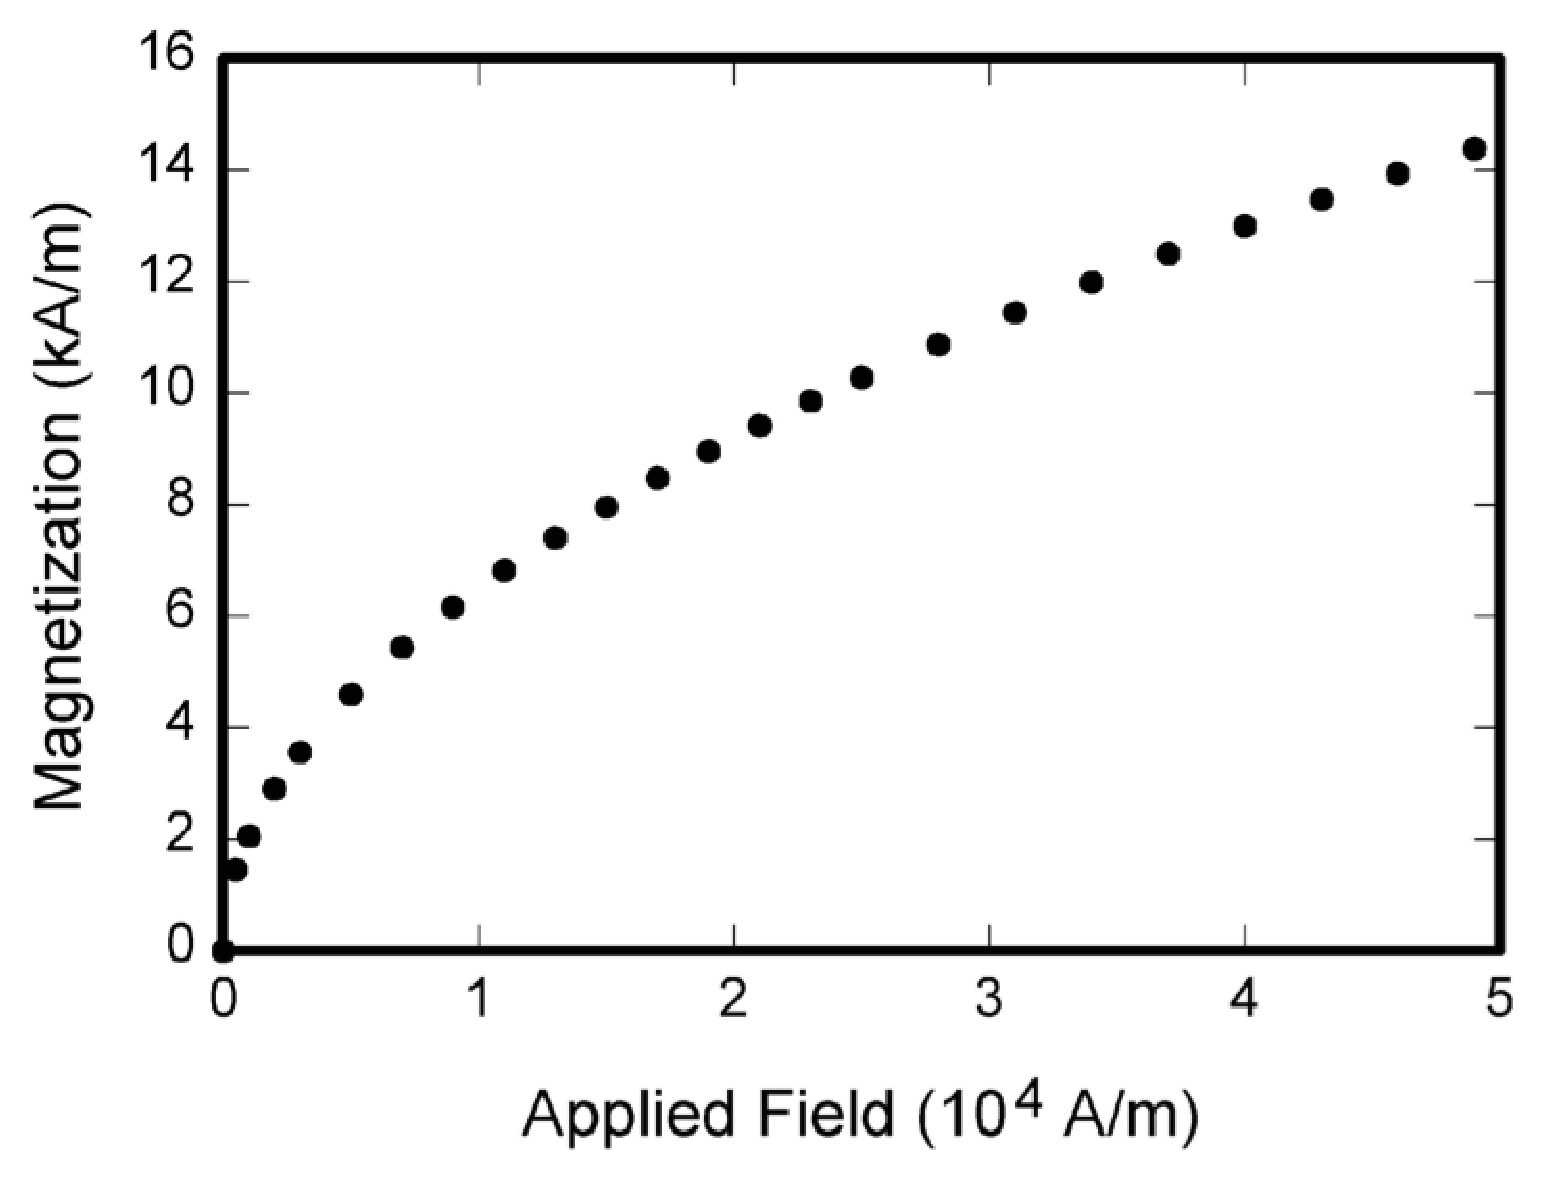
\includegraphics[width=8.5cm]{FIG1.eps}
	\caption{Magnetization as a function of applied field. Note that ``Fig.'' is abbreviated. There is a period after the figure number, followed by two spaces. It is good practice to explain the significance of the figure in the caption.}\label{FIG_1}
\end{figure}


The SI unit for magnetic field strength H is A/m. However, if you wish to use units of T, either refer to magnetic flux density B or magnetic field strength symbolized as \SI{}{\micro0H}. Use the center dot to separate compound units, e.g., ``A�m2.''

\section{Guidelines for Graphics Preparation and Submission}

\subsection{Types of Graphics}
The following list outlines the different types of graphics published in IEEE journals. They are categorized based on their construction, and use of color / shades of gray.

Such figures may include photographs, illustrations, multicolor graphs, and flowcharts.

Figures that are composed of only black lines and shapes. These figures should have no shades or half-tones of gray. Only black and white.

Head and shoulders shots of authors which appear at the end of our papers.  Data charts which are typically black and white, but sometimes include color.

\subsection{Multipart figures}

Figures compiled of more than one sub-figure presented side-by-side, or stacked. If a multipart figure is made up of multiple figure types (one part is lineart, and another is grayscale or color) the figure should meet the stricter guidelines.


\begin{table}[!t]
	\renewcommand{\arraystretch}{1.3}
	\caption{Units for Magnetic Properties}
	\centering
	\label{table_1}
	%\centering
	\resizebox{\columnwidth}{!}{
		\begin{tabular}{l l l}
			\hline\hline \\[-3mm]
			\multicolumn{1}{c}{Symbol} & \multicolumn{1}{c}{Quantity} & \multicolumn{1}{c}{\pbox{20cm}{Conversion from Gaussian and \\ \hphantom{spaces} CGS EMU to $ SI^{a} $ }}  \\[1.6ex] \hline
			$ \Phi $  & magnetic flux & $ 1Mx \rightarrow 10^8 Wb = 10^8 V \cdot s $ \\
			\pbox{20cm}{$ \emph{B} $ \\\hphantom{1}} & \pbox{20cm}{magnetic flux density, \\ \hphantom{1} magnetic induction} &  \pbox{20cm}{$ 1G \rightarrow 10^4 T = 10^4 Wb/m^2 $ \\ \hphantom{1}} \\ 
			$ \emph{H} $ & magnetic field strength & $ 1Oe \rightarrow 10^3/(4\pi)A/m $ \\
			\pbox{20cm}{$ \emph{m} $ \\ \hphantom{1}} & \pbox{20cm}{magnetic moment \\ \hphantom{1}} & \pbox{20cm}{$ 1 erg/G = 1 emu $ \\ \hphantom{1} $ \rightarrow 10^3 A \cdot m^2 = 10^3 J/T $ } \\ 
			\pbox{20cm}{$ \emph{M} $ \\ \hphantom{1}} & \pbox{20cm}{magnetization \\ \hphantom{1}} & \pbox{20cm}{$ 1 erg/(G \cdot cm^3) = 1 emu/cm^3 $ \\ \hphantom{1} $ \rightarrow 10^3 A/m $ } \\ 
			$ 4\pi\emph{M} $ & magnetization & $ 1G \rightarrow 10^3/(4\pi)A/m $ \\
			$ \sigma $ & specific magnetization & $ 1 erg/(G \cdot g) = 1 emu/g \rightarrow 1 A \cdot m^2/kg $ \\
			\pbox{20cm}{$ \emph{j} $ \\ \hphantom{1}} & \pbox{20cm}{magnetic dipole \\ \hphantom{1} moment } & \pbox{20cm}{$ 1 erg/G = 1 emu $ \\ \hphantom{1} $ \rightarrow 4\pi \times 10^{10} Wb \cdot m $ } \\ [1.4ex]
			\pbox{20cm}{$ \emph{J} $ \\ \hphantom{1}} & \pbox{20cm}{magnetic polarization \\ \hphantom{1}} & \pbox{20cm}{$ 1 erg/(G \cdot cm^3) = 1 emu/cm^3 $ \\ \hphantom{1} $ \rightarrow 4\pi \times 10^{4} T $ } \\ 
			$ \chi \ \kappa $ & susceptibility & $ 1 \rightarrow 4\pi $ \\ 
			$ \chi  $ & mass susceptibility & $ 1 cm^3/g \rightarrow 4\pi \times 10^{3} m^3/kg $ \\ 
			\pbox{20cm}{$ \mu $ \\ \hphantom{1}} & \pbox{20cm}{permeability \\ \hphantom{1}} & \pbox{20cm}{$ 1 \rightarrow 4\pi \times 10^{7} H/m $ \\ \hphantom{1} $ =4\pi \times 10^{7} Wb/(A \cdot m) $ } \\ 
			$ \mu_r $ & relative permeability & $ \mu \rightarrow \mu_r $ \\ 
			$ \omega, \emph{W} $ & energy density & $ 1 erg/cm^3 \rightarrow 10^1 J/m^3 $ \\ 
			$ \emph{N}, \emph{D} $ & demagnetizing factor & $ 1 \rightarrow 1/(4\pi) $ \\ [1.4ex]
			\hline\hline
		\end{tabular}
	}
\end{table}

\subsection{File Formats For Graphics}

Format and save your graphics using a suitable graphics processing program that will allow you to create the images as PostScript (PS), Encapsulated PostScript (.EPS), Tagged Image File Format (.TIFF), Portable Document Format (.PDF), or Portable Network Graphics (.PNG) sizes them, and adjusts the resolution settings. If you created your source files in one of the following programs you will be able to submit the graphics without converting to a PS, EPS, TIFF, PDF, or PNG file: Microsoft Word, Microsoft PowerPoint, or Microsoft Excel. Though it is not required, it is recommended that these files be saved in PDF format rather than DOC, XLS, or PPT. Doing so will protect your figures from common font and arrow stroke issues that occur when working on the files across multiple platforms. When submitting your final paper, your graphics should all be submitted individually in one of these formats along with the manuscript.


\subsection{Sizing of Graphics}

Most charts, graphs, and tables are one column wide (3.5 inches / 88 millimeters / 21 picas) or page wide (7.16 inches / 181 millimeters / 43 picas). The maximum depth a graphic can be is 8.5 inches (216 millimeters / 54 picas). When choosing the depth of a graphic, please allow space for a caption. Figures can be sized between column and page widths if the author chooses, however it is recommended that figures are not sized less than column width unless when necessary.

There is currently one publication with column measurements that don't coincide with those listed above. PROCEEDINGS OF THE IEEE has a column measurement of 3.25 inches (82.5 millimeters / 19.5 picas).

The final printed size of author photographs is exactly
1 inch wide by 1.25 inches tall (25.4 millimeters x 31.75 millimeters / 6 picas x 7.5 picas). Author photos printed in editorials measure 1.59 inches wide by 2 inches tall (40 millimeters  x 50 millimeters  / 9.5 picas x 12 picas).


\subsection{Resolution}

The proper resolution of your figures will depend on the type of figure it is as defined in the ``Types of Figures'' section. Author photographs, color, and grayscale figures should be at least 300dpi. Lineart, including tables should be a minimum of 600dpi.


\subsection{Vector Art}

While IEEE does accept, and even recommends that authors submit artwork in vector format, it is our policy is to rasterize all figures for publication. This is done in order to preserve the figures' integrity across multiple computer platforms.


\subsection{Color Space}

The term color space refers to the entire sum of colors that can be represented within the said medium. For our purposes, the three main color spaces are Grayscale, RGB (red/green/blue) and CMYK (cyan/magenta/yellow/black). RGB is generally used with on-screen graphics, whereas CMYK is used for printing purposes.

All color figures should be generated in RGB or CMYK color space. Grayscale images should be submitted in Grayscale color space. Line art may be provided in grayscale OR bitmap colorspace. Note that ``bitmap colorspace'' and ``bitmap file format'' are not the same thing. When bitmap color space is selected, .TIF/.TIFF is the recommended file format.


\subsection{Accepted Fonts Within Figures}

When preparing your graphics IEEE suggests that you use of one of the following Open Type fonts: Times New Roman, Helvetica, Arial, Cambria, and Symbol. If you are supplying EPS, PS, or PDF files all fonts must be embedded. Some fonts may only be native to your operating system; without the fonts embedded, parts of the graphic may be distorted or missing.

A safe option when finalizing your figures is to strip out the fonts before you save the files, creating ``outline'' type. This converts fonts to artwork what will appear uniformly on any screen.


\subsection{Using Labels Within Figures}

\begin{enumerate}
	\item Figure Axis labels\\
	Figure axis labels are often a source of confusion. Use words rather than symbols. As an example, write the quantity``Magnetization,'' or ``Magnetization M,'' not just ``M.'' Put units in parentheses. Do not label axes only with units. As in \mbox{Fig. \ref{FIG_1}}, for example, write ``Magnetization (A/m)'' or ``Magnetization (A m1),'' not just ``A/m.'' Do not label axes with a ratio of quantities and units. For example, write ``Temperature (K),'' not ``Temperature/K.''. Multipliers can be especially confusing. Write ``Magnetization (kA/m)'' or ``Magnetization (103 A/m).'' Do not write ``Magnetization (A/m) x 1000'' because the reader would not know whether the top axis label in \mbox{Fig. \ref{FIG_1}} meant 16000 A/m or 0.016 A/m. Figure labels should be legible, approximately 8 to 10 point type.	
	\item Subfigure Labels in Multipart Figures and Tables\\
	Multipart figures should be combined and labeled before final submission. Labels should appear centered below each subfigure in 8 point Times New Roman font in the format of (a) (b) (c). 	
\end{enumerate}

\subsection{Referencing a Figure or Table Within Your Paper}
When referencing your figures and tables within your paper, use the abbreviation ``Fig.'' even at the beginning of a sentence. Do not abbreviate ``Table.'' Tables should be numbered with Roman Numerals.

\subsection{Checking Your Figures: The IEEE Graphics Checker}
The IEEE Graphics Checker Tool enables authors to pre-screen their graphics for compliance with IEEE Transactions and Journals standards before submission. The online tool, located at \url{http://graphicsqc.ieee.org/}, allows authors to upload their graphics in order to check that each file is the correct file format, resolution, size and colorspace; that no fonts are missing or corrupt; that figures are not compiled in layers or have transparency, and that they are named according to the IEEE Transactions and Journals naming convention. At the end of this automated process, authors are provided with a detailed report on each graphic within the web applet, as well as by email.

For more information on using the Graphics Checker Tool or any other graphics related topic, contact the IEEE Graphics Help Desk by e-mail at graphics@ieee.org.

\subsection{Submitting Your Graphics}
Because IEEE will do the final formatting of your paper, you do not need to position figures and tables at the top and bottom of each column. In fact, all figures, figure captions, and tables can be placed at the end of your paper. In addition to, or even in lieu of submitting figures within your final manuscript, figures should be submitted individually, separate from the manuscript in one of the file formats listed above in section VI-J. Place figure captions below the figures; place table titles above the tables. Please do not include captions as part of the figures, or put them in ``text boxes'' linked to the figures. Also, do not place borders around the outside of your figures.

\subsection{Color Processing / Printing in IEEE Journals}
All IEEE Transactions, Journals, and Letters allow an author to publish color figures on IEEE Xplore� at no charge, and automatically convert them to grayscale for print versions. In most journals, figures and tables may alternatively be printed in color if an author chooses to do so. Please note that this service comes at an extra expense to the author. If you intend to have print color graphics, include a note with your final paper indicating which figures or tables you would like to be handled that way, and stating that you are willing to pay the additional fee.


\section{Conclusion}

A conclusion section is not required. Although a conclusion may review the main points of the paper, do not replicate the abstract as the conclusion. A conclusion might elaborate on the importance of the work or suggest applications and extensions.


\section*{Appendix}

Appendixes, if needed, appear before the acknowledgment.

{\color{red}
\section*{Acknowledgment}

The preferred spelling of the word ``acknowledgment'' in American English out an ``e'' after the ``g.'' Use the singular heading even if you have many acknowledgments. Avoid expressions such as ``One of us (S.B.A.) would like to thank ... .'' Instead, write ``F. A. Author thanks ... .'' In most cases, sponsor and financial support acknowledgments are placed in the unnumbered footnote on the first page, not here.
}

\section*{References and Footnotes}

\subsection{References}
References need to be cited in text. Put the number on the line, in square brackets inside the punctuation.  Multiple references are each numbered with separate brackets. When citing a section in a book, please give the relevant page numbers. In text, refer simply to the reference number. Do not use ``Ref.'' or ``reference'' except at the beginning of a sentence: ``Reference [\#] shows ... .'' Please do not use automatic endnotes in Word, rather, type the reference list at the end of the paper using the ``References'' style.

Reference numbers are set flush left and form a column of their own, hanging out beyond the body of the reference. The reference numbers are on the line, enclosed in square brackets. In all references, the given name of the author or editor is abbreviated to the initial only and precedes the last name. Use them all; use et al. exceptionally if more than 6 author names were listed. Use commas around Jr., Sr., and III in names. Abbreviate conference titles \cite{inproceedings1}.  When citing journals \cite{article1, article2}, provide the issue number, page range, volume number, DOI, year, and/or month if available. When referencing a patent \cite{patent1}, provide the day and the month of issue, or application. References may not include all information; please obtain and include relevant information. Do not combine references. There must be only one reference with each number. If there is a URL included with the print reference, it can be included at the end of the reference \cite{onlinebook1}.

Authors are encouraged to include the DOI number for each reference. It's the most important part of the reference. The DOI is like a digital fingerprint and it's used to identify the article without mistakes.

Other than books \cite{inbook1, book1}, capitalize only the first word in a paper title, except for proper nouns and element symbols. For papers published in translation journals, please give the English citation first, followed by the original foreign-language citation See the end of this document for formats and examples of common references. For a complete discussion of references and their formats, see ``The IEEE Style Manual,'' available as a PDF link off the Author Digital Toolbox main page.

\subsection{Footnotes}
Number footnotes separately in superscripts (Insert | Footnote).\footnote{It is recommended that footnotes be avoided (except for the unnumbered footnote with the receipt date on the first page). Instead, try to integrate the footnote information into the text.}  Place the actual footnote at the bottom of the column in which it is cited; do not put footnotes in the reference list (endnotes). Use letters for table footnotes  (see \mbox{Table \ref{table_1}}).


\section{Editorial Policy}

Do not submit a reworked version of a paper you have submitted or published elsewhere. Do not publish ``preliminary'' data or results. The submitting author is responsible for obtaining agreement of all coauthors and any consent required from sponsors before submitting a paper.

The IEEE Transactions and Journals Department does not publish conference records or proceedings. The department  does publish papers related to conferences that have been recommended for publication on the basis of peer review. As a matter of convenience and service to the technical community, these topical papers are typically collected and published in one special issue of most transactions publications.

At least two reviews are required for every paper submitted. Indecipherable English is a valid reason for rejection. There is a service available that will help you improve your English for a fee, and the link to that service can be found at \url{http://www.ieee.org/web/publications/authors/transjnl/index.html}.

Authors of rejected papers may revise and resubmit them as regular papers, whereupon they will be reviewed by two new referees.

\section{Publication Principles}

The two types of contents of that are published are; 1) peer-reviewed and 2) archival. The Transactions and Journals Department publishes scholarly articles of archival value as well as tutorial expositions and critical reviews of classical subjects and topics of current interest.
Authors should consider the following points:

\begin{enumerate}[1)]
\item Technical papers submitted for publication must advance the state of knowledge and must cite relevant prior work.
\item The length of a submitted paper should be commensurate with the importance, or appropriate to the complexity, of the work. For example, an obvious extension of previously published work might not be appropriate for publication or might be adequately treated in just a few pages.
\item Authors must convince both peer reviewers and the editors of the scientific and technical merit of a paper; the standards of proof are higher when extraordinary or unexpected results are reported.
\item Because replication is required for scientific progress, papers submitted for publication must provide sufficient information to allow readers to perform similar experiments or calculations and use the reported results. Although not everything need be disclosed, a paper must contain new, useable, and fully described information. For example, a specimen's chemical composition need not be reported if the main purpose of a paper is to introduce a new measurement technique. Authors should expect to be challenged by reviewers if the results are not supported by adequate data and critical details.
\item Papers that describe ongoing work or announce the latest technical achievement, which are suitable for presentation at a professional conference, may not be appropriate for publication.
\end{enumerate}



% References

\bibliographystyle{Bibliography/IEEEtranTIE}
\bibliography{Bibliography/IEEEabrv,Bibliography/BIB_1x-TIE-2xxx}\ %IEEEabrv instead of IEEEfull

{\color{red}
	
\vspace{-1cm}
\begin{IEEEbiography}[{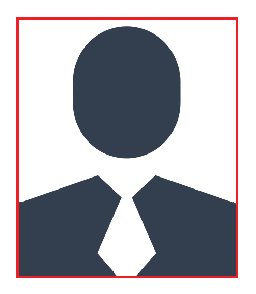
\includegraphics[width=1in,height=1.25in,clip,keepaspectratio]{photo-men.eps}}]
{First A. Author1} and the other authors may include biographies at the end of regular papers. The first paragraph may contain a place and/or date of birth (list place, then date). Next, the author's educational background is listed. The degrees should be listed with type of degree in what field, which institution, city, state or country, and year degree was earned. The author's major field of study should be lower-cased.

The second paragraph uses the pronoun of the person (he or she) and not the author's last name. It lists military and work experience, including summer and fellowship jobs. Job titles are capitalized. The current job must have a location; previous positions may be listed without one. Information concerning previous publications may be included.

The third paragraph begins with the author's title and last name (e.g., Dr. Smith, Prof. Jones, Mr. Kajor, Ms. Hunter). List any memberships in professional societies other than the IEEE. Finally, list any awards and work for IEEE committees and publications. If a photograph is provided, the biography will be indented around it. The photograph is placed at the top left of the biography. Personal hobbies will be deleted from the biography.
\end{IEEEbiography}

\vspace{-2cm}
\begin{IEEEbiography}[{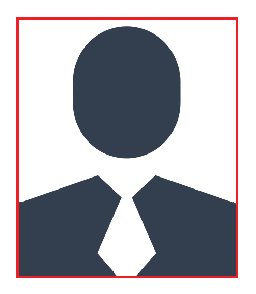
\includegraphics[width=1in,height=1.25in,clip,keepaspectratio]{photo-men.eps}}]
{Second B. Author2} (M'12) was born in City, Country. He received the M. degree in electrical engineering from University of City, Country in 2012.

The second paragraph uses the pronoun of the person (he or she) and not the author's last name. It lists military and work experience, including similar information to the previous author, including military, work experience, and other jobs. Job titles are capitalized. The current job must have a location; previous positions may be listed without one. Information concerning previous publications may be included.

The third paragraph begins with the author's title and last name (e.g., Dr. Smith, Prof. Jones, Mr. Kajor, Ms. Hunter), including similar information to the previous author, including the list of any awards and work for IEEE committees and publications. The photograph is placed at the top left of the biography. Personal hobbies will be deleted from the 
biography.\\ 
\end{IEEEbiography}

\vspace{-2cm}
\begin{IEEEbiography}[{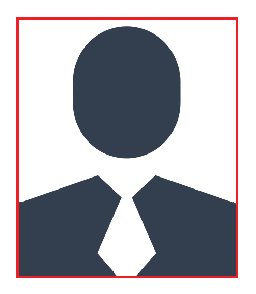
\includegraphics[width=1in,height=1.25in,clip,keepaspectratio]{photo-men.eps}}]
{Third C. Author3} (M'99-SM'04-F'09) was born in City, Country. He received the M. and SM. and F. degrees in electrical engineering from University of City, Country in 1999, 2004 and 2009 respectively.

The second paragraph uses the pronoun of the person (he or she) and not the author's last name. It lists military and work experience, including similar information to the previous author, including military, work experience, and other jobs.

The third paragraph begins with the author's title and last name (e.g., Dr. Smith, Prof. Jones, Mr. Kajor, Ms. Hunter), including similar information to the previous author, including the list of any awards and work for IEEE committees and publications. The photograph is placed at the top left of the biography. Personal hobbies will be deleted from the biography.
\\ \\ 
\end{IEEEbiography}

}

\end{document}
